\documentclass{fenicscourse}

\begin{document}

\fenicslecture{Overview}
              {Martin Aln\ae{}s}

\begin{frame}
  \frametitle{Course outline}

  % Note to lecturers: use \textcolor{grey}{Lecture title} to mark
  % lectures that are not included in a course

  \small

% 0900 Outline
% 0930 L02 Static linear PDEs
% 1000 Coffee
% 1015 Hands-on L02
% 1130 L03 Time-dependent
% 1200 Lunch
% 1230 Hands-on L03
% 1315 L05
% 1345 Coffee
% 1400 L06
% 1430 Hands-on
% 1500 The End

% Time: 2.5h * 4
%

  \begin{enumerate}
  \item[L00]
    \textcolor{grey}{Introduction to FEM}
  \item[L01]
    \textcolor{grey}{Introduction to FEniCS}
  \item[L02]
    Static linear PDEs
  \item[L03]
    Static nonlinear PDEs
  \item[L04]
    Time-dependent PDEs
  \item[L05]
    \textcolor{grey}{Happy hacking: Tools, tips and coding practices}
  \item[L06]
    Static hyperelasticity
  \item[L07]
    \textcolor{grey}{Dynamic hyperelasticity}
  \item[L08]
    The Stokes problem
  \item[L09]
    Incompressible Navier--Stokes
  \item[L10]
    \textcolor{grey}{Discontinuous Galerkin methods for elliptic equations}
  \item[L11]
    \textcolor{grey}{A posteriori error estimates and adaptivity}
  \end{enumerate}

  \normalsize

  {\footnotesize Lectures can be downloaded from
    \url{http://fenicsproject.org/pub/course/}}

\end{frame}


% The quickest FEniCS intro
\begin{frame}
\medskip

\includegraphics[width=0.99\textwidth]{png/fenics_banner.png}
\begin{columns}[c]
\begin{column}{0.4\textwidth}
\bf{The FEniCS Project is a collection of open-source software
  components aimed at the numerical solution of partial differential
  equations using finite element methods}
\end{column}
\begin{column}{0.7\textwidth}
  \begin{block}{Key distinguishing features}
  \begin{itemize}
  \item
    FEniCS (Python/C++) code is quick to write and easy to read
  \item
    `Any' finite element formulation of 'any' partial differential
    equation can be coded
  \item
    Automated code generation is heavily used under the hood to
    create efficient, specialized, low-level code
  \item
    Performance -- implicit problems with over $12\, 000\, 000\, 000$
    degrees of freedom can be solved in a couple of minutes
  \end{itemize}
  \end{block}
\end{column}
\end{columns}
  \begin{center}
    \colemph{\url{http://fenicsproject.org/}}
  \end{center}
\end{frame}

\begin{frame}
\frametitle{FEniCS has been used for a wide range of
  equations and applications}

{\tiny Reaction-diffusion equations; Stokes with or without nonlinear
  viscosity; compressible and incompressible Navier--Stokes; RANS
  turbulence models; shallow water equations; Bidomain equations;
  nonlinear and linear elasticity; nonlinear and linear
  viscoelasticity; Schr\"odinger; Biot's equations for porous media,
  fracture mechanics, electromagnetism, liquid crystals including
  liquid crystal elastomers, combustion, ... and coupled systems of
  the above, ...}

\begin{center}
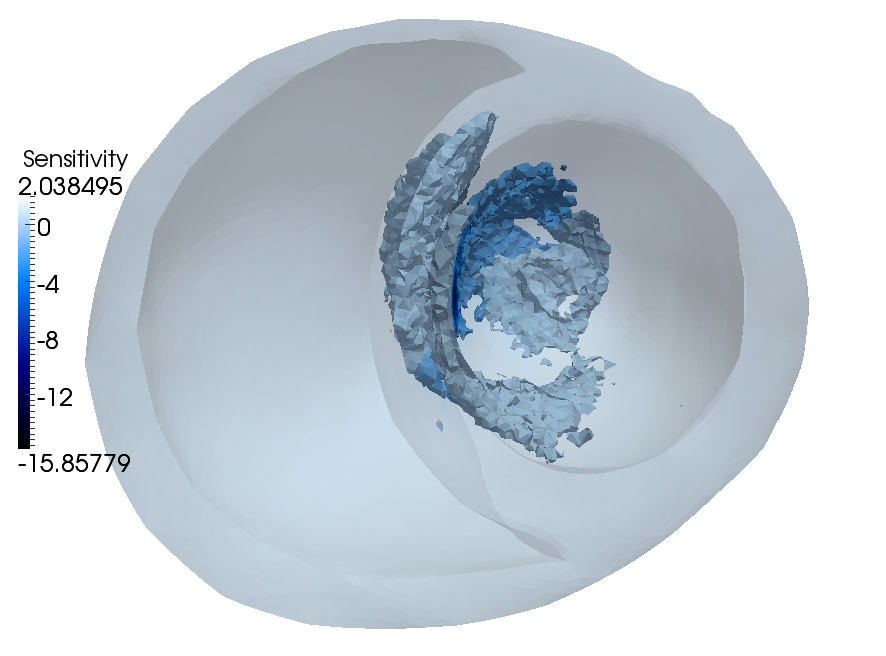
\includegraphics[width=0.24\textwidth]{png/g_el_plusx.png}
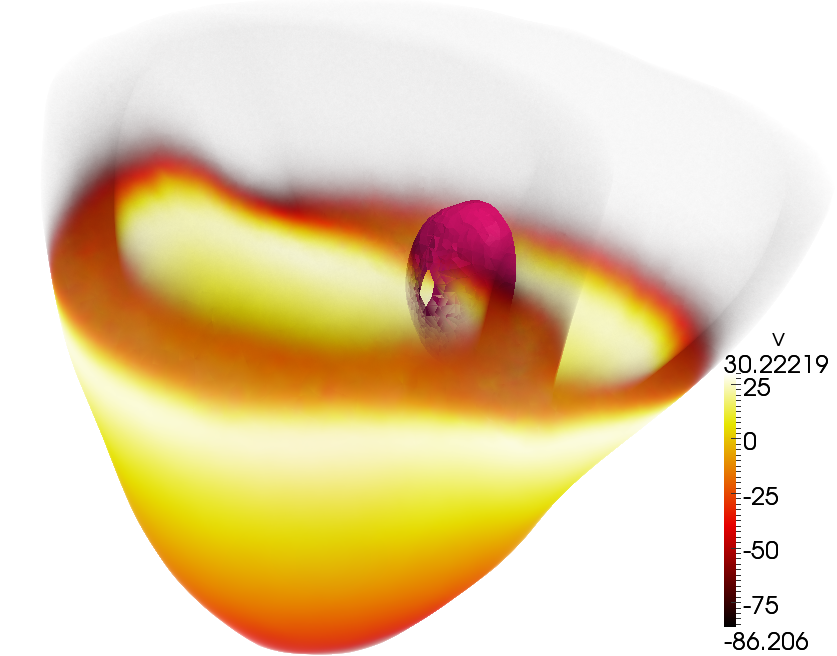
\includegraphics[width=0.24\textwidth]{png/unhealthy_v_at_T200.png}
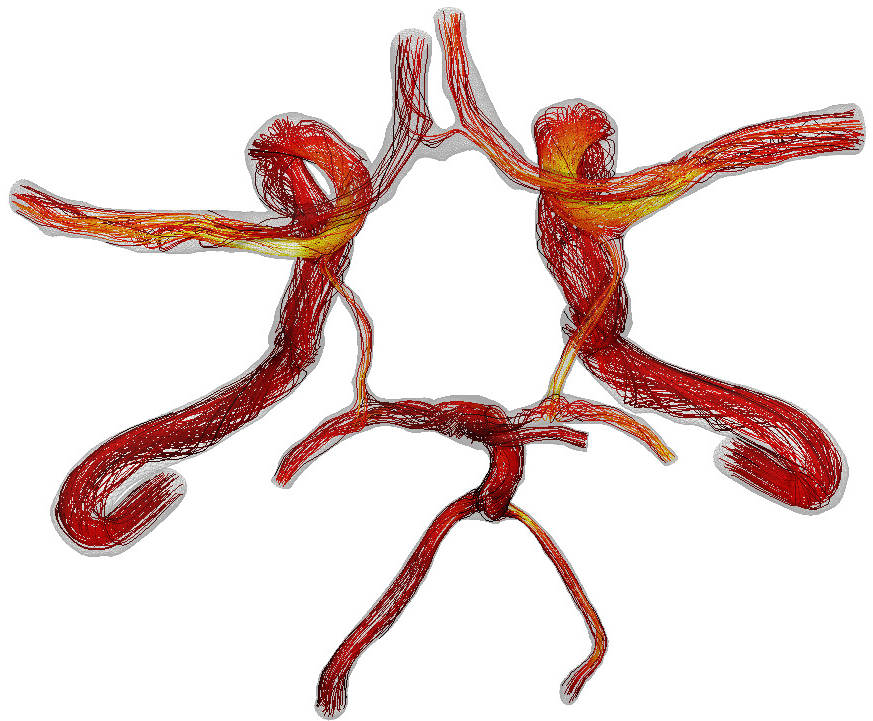
\includegraphics[width=0.24\textwidth]{png/circle_of_willis_simulation.png}
\end{center}

{\tiny for simulating blood flow, computing calcium release in cardic
  tissue, computing the cardiac potential in the heart, simulating
  mantle convection, simulating melting ice sheets, computing the
  optimal placement of tidal turbines, simulating and reconstructing
  tsunamis, simulating the flow of cerebrospinal fluid and the
  deformation of the spinal cord, simulating waveguides, ... }

\end{frame}


% Show a simple taster
\begin{frame}
  \frametitle{Hello World in FEniCS: problem formulation}

  \begin{block}{Poisson's equation}
    \vspace{-0.5cm}
    \begin{displaymath}
      \begin{split}
        -\Delta u &= f \quad \mbox{ in } \Omega \\
        u &= 0 \quad \mbox { on } \partial\Omega
      \end{split}
    \end{displaymath}
  \end{block}

  \begin{block}{Finite element formulation}
    \vspace{1ex}
    Find $u \in V$ such that
    \begin{displaymath}
      \underbrace{\int_{\Omega} \nabla u \cdot \nabla v \dx}_{\textcolor{fenicsred}{a(u,v)}}
      = \underbrace{\int_{\Omega} f \, v \dx}_{\textcolor{fenicsred}{L(v)}}
      \quad \foralls v \in V
    \end{displaymath}
  \end{block}

\end{frame}

\begin{frame}[fragile]
  \frametitle{Hello World in FEniCS: implementation}

    \begin{python}
from fenics import *

mesh = UnitSquareMesh(32, 32)

V = FunctionSpace(mesh, "Lagrange", 1)
u = TrialFunction(V)
v = TestFunction(V)
f = Expression("x[0]*x[1]", degree=2)

a = dot(grad(u), grad(v))*dx
L = f*v*dx

bc = DirichletBC(V, 0.0, DomainBoundary())

u = Function(V)
solve(a == L, u, bc)
plot(u)
    \end{python}

\end{frame}

\begin{frame}
  \frametitle{Basic API}

  \begin{itemize}
  \item
    \texttt{Mesh},
    \texttt{Vertex},
    \texttt{Edge},
    \texttt{Face},
    \texttt{Facet},
    \texttt{Cell}
  \item
    \texttt{FiniteElement}, \texttt{FunctionSpace}
  \item
    \texttt{TrialFunction},
    \texttt{TestFunction},
    \texttt{Function}
  \item
    \texttt{grad()}, \texttt{curl()}, \texttt{div()}, \ldots
  \item
    \texttt{Matrix}, \texttt{Vector}, \texttt{KrylovSolver}, \texttt{LUSolver}
  \item
    \texttt{assemble()}, \texttt{solve()}, \texttt{plot()}
  \end{itemize}

  \vspace{1cm}

  \begin{itemize}
  \item
    Python interface generated semi-automatically by SWIG
  \item
    C++ and Python interfaces almost identical
  \end{itemize}

\end{frame}


% Learning more than what this course covers
%\begin{frame}
    \frametitle{Sounds great, but how do I find my way through the
    jungle?}
    \begin{center}
        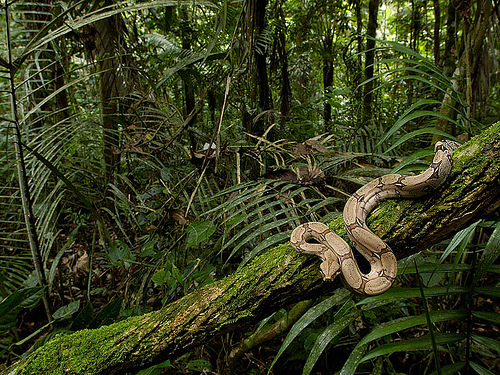
\includegraphics[width=0.8\textwidth]{jpg/jungle10.jpg}
    \end{center}
\end{frame}

\begin{frame}
    \frametitle{Three survival advices}
    \begin{columns}[c]
        \begin{column}{0.33\textwidth}
            \begin{center}
                
\includegraphics[width=0.99\textwidth]{png/python_logo.png}
            \end{center}
        \end{column}
        \begin{column}{0.33\textwidth}
            \begin{center}
                
\includegraphics[width=0.99\textwidth]{jpg/documentation.jpg}\\
            \end{center}
        \end{column}
        \begin{column}{0.33\textwidth}
            \begin{center}
                
\includegraphics[width=0.99\textwidth]{jpg/question-blue.jpg}
            \end{center}
        \end{column}
    \end{columns}
    \begin{columns}[t]
        \begin{column}{0.33\textwidth}
            \begin{center}
                \colemph{Use the right Python tools}
            \end{center}
        \end{column}
        \begin{column}{0.33\textwidth}
            \begin{center}
                \colemph{Explore the documentation}
            \end{center}
        \end{column}
        \begin{column}{0.33\textwidth}
            \begin{center}
                \colemph{Ask, report and request}
            \end{center}
        \end{column}
    \end{columns}
\end{frame}


% TODO: Update webpage images when readthedocs work is completed

% Demos on old page
\begin{frame}
  \begin{center}
     {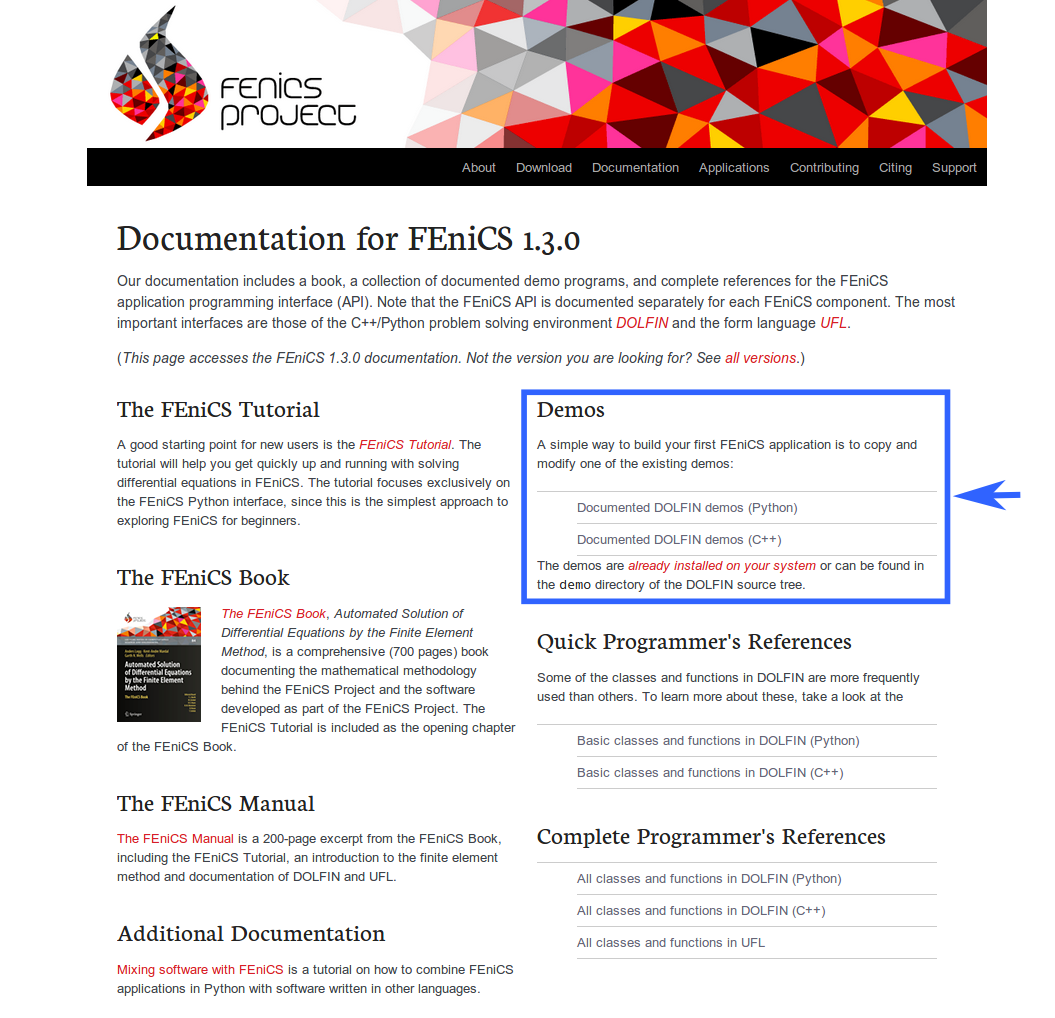
\includegraphics[width=0.80\textwidth]{png/fenics-doc-webpage-5.png}}
    \small
    \colemph{\url{http://fenicsproject.org/documentation/}}
  \end{center}
\end{frame}

% Reference docs on old page
\begin{frame}
  \begin{center}
     {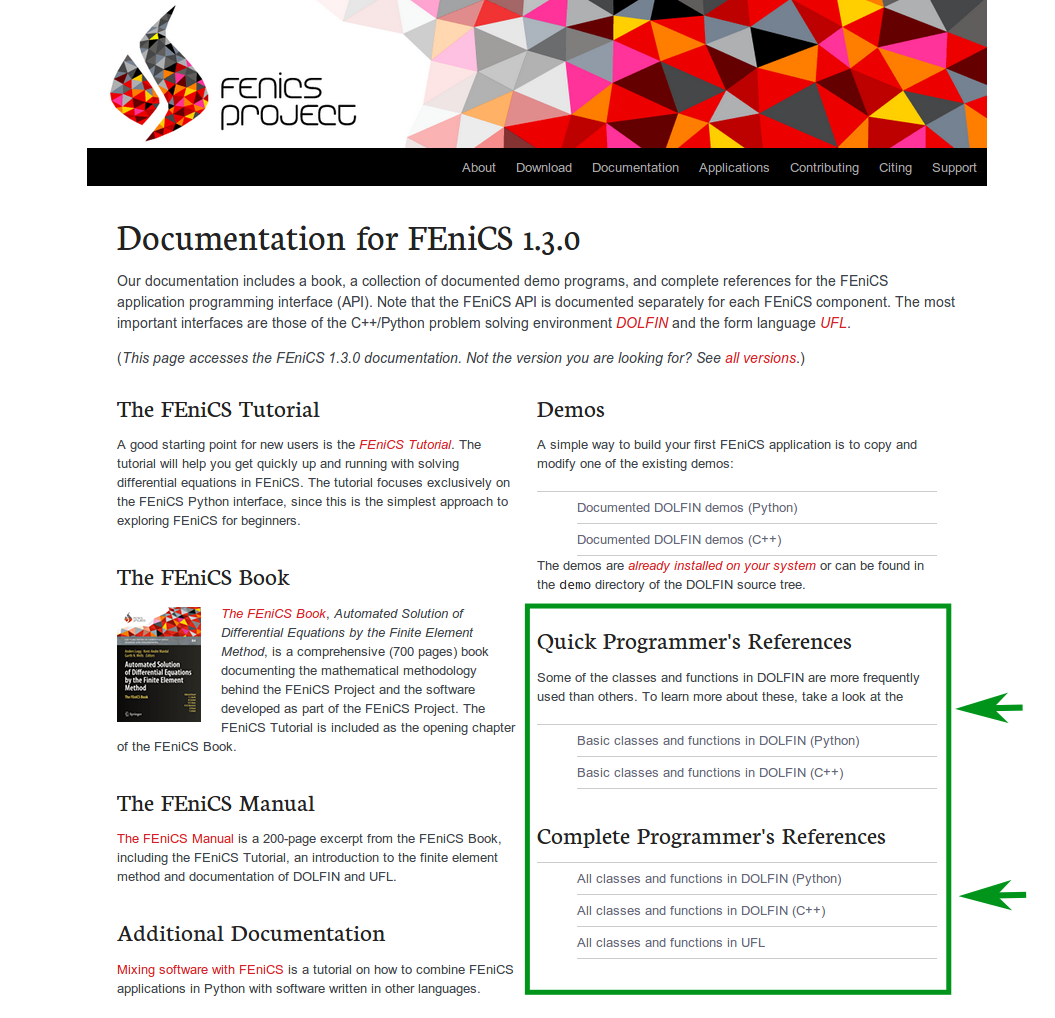
\includegraphics[width=0.80\textwidth]{png/fenics-doc-webpage-6.png}}
    \small
    \colemph{\url{http://fenicsproject.org/documentation/}}
  \end{center}
\end{frame}

% Currently migrating
\begin{frame}
  \begin{center}
     {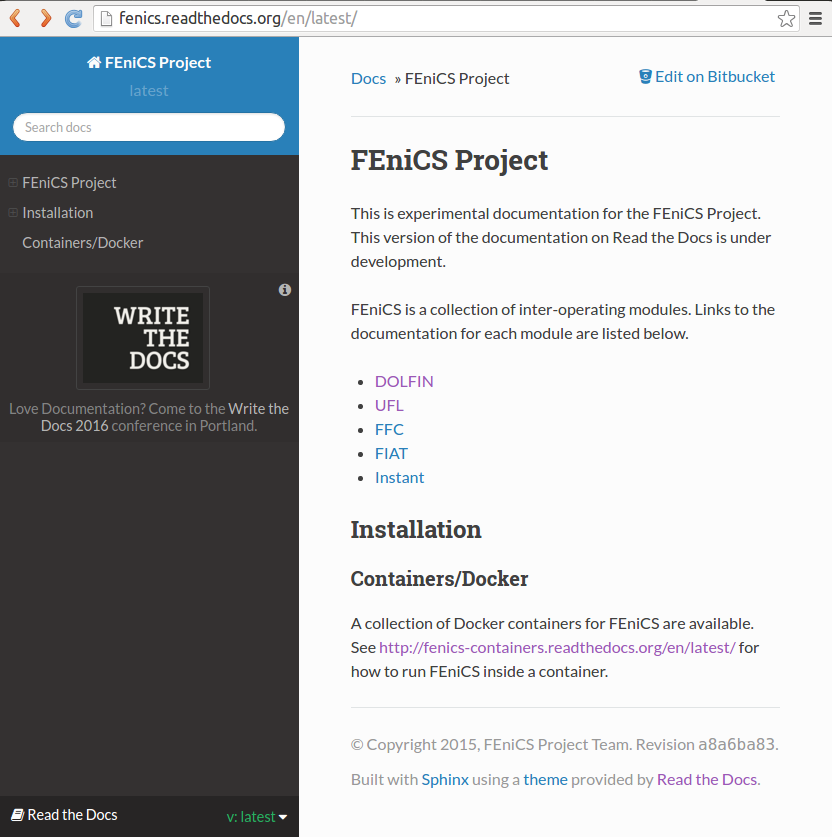
\includegraphics[width=0.80\textwidth]{png/fenics-readthedocs-webpage-1.png}}
    \small
    \colemph{\url{http://fenics.readthedocs.org/}}
  \end{center}
\end{frame}

\begin{frame}
    \frametitle{Development community is organized via bitbucket.org}
    \begin{center}
        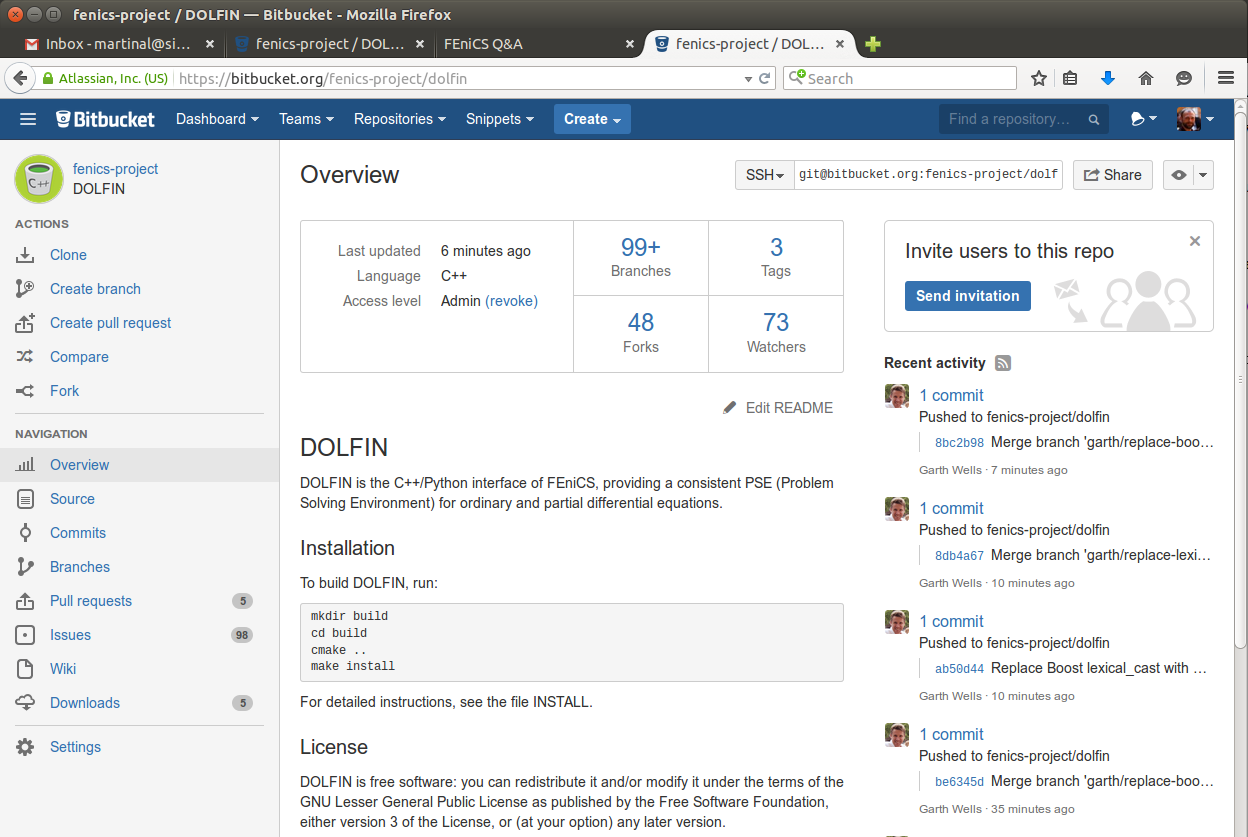
\includegraphics[height=0.75\textheight]{png/fenics-bitbucket-webpage.png}
        \vspace{1em}
        \small
        \colemph{\url{http://bitbucket.org/fenics-project/}}
    \end{center}
\end{frame}
\begin{frame}
    \frametitle{Community help is available via QA forum}
    \begin{center}
        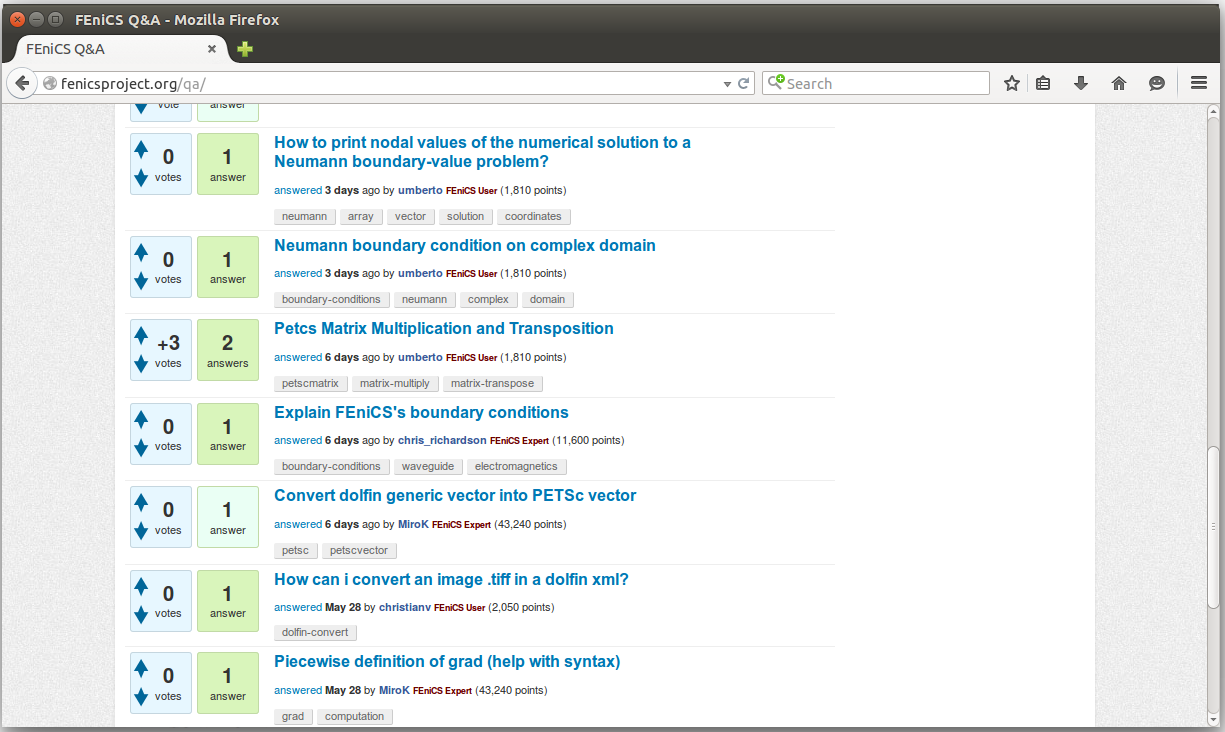
\includegraphics[width=1.0\textwidth,height=0.7\textheight]{png/fenics-qa-website.png}
        \vspace{1em}
        \small
        \colemph{\url{https://fenicsproject.org/qa}}
    \end{center}
\end{frame}


% Installation
\begin{frame}
  \frametitle{Installation alternatives}

  % FEniCS uses standard setup.py and cmake tools
  % but dependencies are tricky to configure.

  \begin{tabular}{cp{10cm}}
    
\includegraphics[height=1cm]{png/docker_logo.png} &
    \begin{minipage}{10cm}
      \ding{43} Docker images on Linux, Mac, Windows
      \vspace{0.6cm}
    \end{minipage}
    \\
    
\includegraphics[height=1cm]{png/source.png} &
    \begin{minipage}{10cm}
      \ding{43} Build from source with Hashdist (fenics-install.sh)
      \vspace{0.8cm}
    \end{minipage}
    \\
    
\includegraphics[height=1cm]{png/ubuntu_logo.png} &
    \begin{minipage}{10cm}
      \ding{43} PPA with apt packages for Debian and Ubuntu
      \vspace{0.6cm}
    \end{minipage}
    \\
    
\includegraphics[height=1cm]{png/mac_osx_logo.png} &
    \begin{minipage}{10cm}
      \ding{43} Drag and drop installation on Mac OS X
      \vspace{0.8cm}
    \end{minipage}
  \end{tabular}

  \begin{center}
    \colemph{\url{http://fenicsproject.org/download/}}
  \end{center}

\end{frame}

\begin{frame}[fragile]
  \frametitle{Installation using Docker}

%Docker allows defining and \emph{image} of prebuilt complex software
%setups and running this inside a \emph{container} which is a fully
%isolated environment that does not interfere with the rest of your
%computer. We provide several different images containing FEniCS and
%dependencies.

Follow instructions to install Docker on linux, mac, or windows:
  \begin{center}
    \colemph{\url{https://docs.docker.com/linux/}} or \url{mac/}, \url{windows/}
  \end{center}

Download and open a terminal in a clean FEniCS environment:
  \begin{bash}
$ docker run -ti quay.io/fenicsproject/dev
  \end{bash}

More instructions on using FEniCS Docker images here:
  \begin{center}
    \colemph{\url{http://fenics-containers.readthedocs.org}}
  \end{center}

\end{frame}

\begin{frame}[fragile]
  \frametitle{Installation using Docker+fenicsproject script}

Install Docker, then get the fenicsproject script:
  \begin{bash}
$ curl -s http://get.fenicsproject.org | sh
  \end{bash}

Now you can initialize and run in a clean FEniCS environment simply with:
  \begin{bash}
$ fenicsproject create myfenics dev
$ fenicsproject start myfenics
  \end{bash}

Or start a Jupyter notebook in a clean environment with:
  \begin{bash}
$ fenicsproject notebook mynotebook dev-py3
$ fenicsproject start mynotebook
  \end{bash}

\end{frame}



\begin{frame}[fragile]
{In this course we'll be running on a local Jupyter Notebook server}
\begin{itemize}
\item Open \texttt{nike.simula.no} in a webbrowser
\item Click ``New'', ``Python 3''
\item Try entering some code:
\end{itemize}
\begin{python}
from fenics import *

%matplotlib inline
parameters["plotting_backend"] = "matplotlib"

mesh = UnitCubeMesh(16, 16, 16)
plot(mesh)
\end{python}
\end{frame}


\begin{frame}{Let's get started and remember:}

\linespread{2.0}
\bigskip
\begin{itemize}
\item
{\footnotesize \textbf{Lectures} can be downloaded from
  \url{http://fenicsproject.org/pub/course/lectures}}

\item
{\footnotesize \textbf{Data} for exercises can be downloaded from
  \url{http://fenicsproject.org/pub/course/data}}

\item
{\footnotesize \textbf{Solutions} for exercises can be downloaded from
  \url{http://fenicsproject.org/pub/course/src} \\
(Secret password needed!)
}
\end{itemize}
\linespread{1.0}\

\end{frame}


\end{document}
